\documentclass{article}

% \usepackage{nips_2018} % ready for submission
% \usepackage[preprint]{nips_2018} % compile a preprint version
% \usepackage[final]{nips_2018} % to compile a camera-ready version
% \usepackage[nonatbib]{nips_2018} % to avoid loading the natbib package
\usepackage[preprint, nonatbib]{nips_2018}

\usepackage{graphicx}
\graphicspath{ {./images/} }
\usepackage{subfig}
\usepackage{color,soul}
\usepackage[utf8]{inputenc} % allow utf-8 input
\usepackage[T1]{fontenc}    % use 8-bit T1 fonts
\usepackage{hyperref}       % hyperlinks
\usepackage{url}            % simple URL typesetting
\usepackage{booktabs}       % professional-quality tables
\usepackage{amsfonts}       % blackboard math symbols
\usepackage{microtype}      % micro-typography
\usepackage{cite}
\usepackage{color}
\usepackage{algorithmicx}
\title{Proactive Caching with Deep Reinforcement Learning}

\author{
  HONG Yuncong \\
  Department of Computer Science \\
  The University of Hong Kong \\
  \texttt{ychong@cs.hku.hk} \\
  \And % Using \AND forces a line break at that point
  ZENG Qunsong \\
  Department of Electrical and Electronic Engineering \\
  The University of Hong Kong \\
  \texttt{qszeng@eee.hku.hk} \\
}

\begin{document}

\maketitle

\begin{abstract}
  With the development of cache technology, the performance of real-time networks keeps increasing. The traditional designs for cache placement problem ordinarily employ simple online algorithms, resulting in limitations of solvable problem domain. In this paper, we consider a complicated dynamic programming problem, which is difficult to be solved efficiently with the traditional algorithms. Here, we propose to solve the caching placement problem within acceptable time with deep reinforcement learning (DRL). The performance of our implementations will be evaluated with the real users' data from Google.
\end{abstract}

\begin{section}{Introduction}
    \label{intro}
    Caching is a widely used technology in system to reduce the load on access communication links and shorten access time to the selected contents \cite{general-cache}. This technique is often aimed at caching the contents from the cloud server in advance. In this particular way, the time and resources needed to request and transport contents from upper level cloud server can be effectively saved.
    
    As for caching placement problem, one practical design is content delivery network (CDN) which is a network of servers linked together in order to deliver contents with high performance \cite{cloudflare}. Emerging areas, such as information centric networks (ICNs) and cloud computing frameworks, \cite{ref1,ref2,ref3,ref4} are based on caching problem and are attracting researchers' attention. Many algorithms for caching placement problems are elaborated in related works \cite{dl-mec,dl-icn,expert-cdn}.
    
    However, with content caching rises the policy control problem, in which we have to explore and decide which contents to store in caches \cite{DBLP:journals/corr/abs-1712-08132}. Although many related works have exploited their algorithms, few of them can adapt to the online production environment with complicated control problem very well. Inspired by deep reinforcement learning method, we propose to design a DRL algorithm for caching decisions. Our concern in this proposal is to formulate the basic frame for cache hit rate, cache replacement cost and communication cost, and to train a neural network to select the optimal online placement decision for cache nodes.
\end{section}

\begin{section}{Background}
    \label{background}
    In this section, \dots
\end{section}

\begin{section}{Related Works}
    \label{review}
    In this section, \dots
\end{section}

\begin{section}{Formulation}
    \label{formulation}
    We consider the scenario that one single user continuously request a finite set of files from one single edge node. The request would demand one file consisted of segments one time, and there are fixed known file set for that user on the cache node.
    This proposed problem could be considered as taken apart from a more complex model. As the cache node is with finite coverage to server the mobile devices, the mobile users could find finite number of edge cache nodes around. The generalized protocol for association could be: One mobile users firstly initiate the \textit{association request} with all of the cache nodes it could "see", then associate with the best one which accepts the request; the cache node then reserve storage space according to user's quota for service, and thus independent from other users' request response.
    
    In the following sections, we will firstly elaborate the network model and caching model for our problem, and then we come up with the formal problem definition in the last section.

    \subsection{Network Model}
    \label{net_model}
    In our model, other than edge nodes and mobile users, there exists one centralized storage entity called \emph{Cloud} to store all the files users previously uploaded.
    The network model is illustrated in the following figure \ref{fig:network}:

    \begin{figure}[h!]
        \label{fig:network}
        \centering
        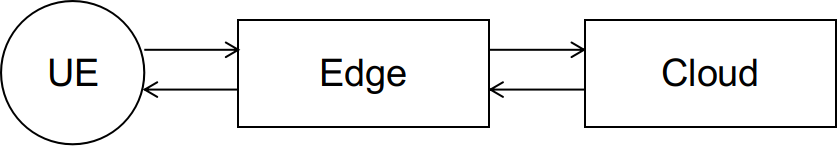
\includegraphics[width=0.8\linewidth]{images/network.png}
        \caption{Network Model for Caching Problem}
    \end{figure}

    The link between Edge Node and Cloud is called "backhaul link", and the link between Edge node and UE (User Equipment) is called "fronthaul link".
    As we consider the scenario with edge caching, it's reasonable that the delay of fronthaul link is rather fixed only caused by bandwidth restriction. The mobile user (UE) should be allocated with enough communication bandwidth with the support of the initialization procedure, as what we have talked about in the beginning. The backhaul is always assumed with large bandwidth supported by the backbone network, and the propagation and processing delay compose the major factors of the total link-wide delay.

    Furthermore, we denote the the fronthaul delay with a constant $T_0$ as it's rather negligible compared with the backhaul delay. Then we denote the pseudo-backhaul bandwidth with a random variable $BW^{back}$, which could be estimated with large enough on-system data samples in the backbone network.
    
    \subsection{Caching Model}
    As for the caching procedure we described, there are just general files stored encoded in binary format. We consider that files are stored into segments on both Edge and Cloud side, which is easy to quantize the different length of files.The storage capacity of edge cache node is bounded considering energy efficiency and volume limit. But the storage on cloud is assumed to be incredible large.
    
    The files are stored in segments on cloud and each segment is with the same size. The storage is continuous with all the file segments aligned head-to-tail; and for each file, we assume there is one oracle (or called \textit{function}), $\mathcal{D}$ to query the starting and ending index for a certain file.

    However, the transmission time of the fixed-size segments could not be quantized due to the varied transmission delay on backhaul link. The integrity of the received segments is guaranteed by error-correction coding scheme and is not considered in our formulation. And due to the error-correction assumption, the fragment of a segment is meaningless and could not recover the original information without fully received.

    \subsection{Request Problem Definition}
    With the Network and Cache model elaborated above, here we give the description of the whole problem.

    We assume that there are total $N$ files for that user, and the file set is denoted as $\mathcal{F} = \{f_1, f_2, \dots, f_N\}$. Each file is composed of different number of segments, and stored continuously head-to-tail on cloud according to the index as:
    $$
    \mathcal{S_F} = \{S_{1,1}, \dots, S_{1,|f_1|}, \dots, S_{N,1}, \dots, S_{N,|f_n|}\}
    $$
    where $|f_i|$ is the number of segments of $i$-th file, and each segment $S_{i,j}$ is of same size denoted as $l_0$. For convenience of expression, we further define the public query oracle that:
    $$
    \mathcal{D}:f_i \to \{S_{f_i,1}, \dots, S_{f_i,|f_i|}\}, \forall f_i \in \mathcal{F}
    $$
    which is accessible from both Edge and Cloud to obtain the segments set of $i$-th file. The storage capacity of the cache node is denoted as $C$ segments, which is considered rather smaller compared with number of the total file segments.

    The request process $\mathcal{R}(t)$ could be divided into multiple episode, which means that the request could only in initiated after the previous request is been served, as we don't allow batched request in our problem. When one request happens, the cache node should firstly ask the oracle $\mathcal{D}$ to obtain the knowledge of segments set to serve. Then the Edge Node divided the requested segments set into two subset according to the storage: $\mathcal{S}_R^{1}$ for hit segments, $\mathcal{S}_R^{0}$ for missing segments.
    The cache node could serve $\mathcal{S}_R^{1}$ with local hit segments each with fixed delay $T_0$ defined in \ref{net_model}. And the time consumed for $\mathcal{S}_R^{0}$ is what we want to minimize because we notice that the service time is heavily affected from the previous storage state.

    We denote the proactive caching policy set as $\mathcal{A} =\mathcal{F} \times \mathcal{S}$, which implies the complexity of potential action space is non-linear. And then we could formulate stochastic optimization problem as following:
    $$
    \min_{\mathcal{A}} \lim_{T \to \infty} \frac{1}{T} E[\sum_r^{\mathcal{R}(t)} \frac{|\mathcal{S}_{r}^{0}|}{BW^{back}(t)}]
    $$
    which implies that the optimization target is to minimize the average service time for missing segments over all the time. The metric of service time is better than conventional git rate cause the varied delay of backhaul also affects the user experience. And for this stochastic optimization problem, we need powerful algorithm to predict the action with respect to request and delay distribution in real-time.

    In the following chapter, we will formulate this optimization problem as deep reinforcement learning problem, and leverage an existing scheme called A3C to solve the proactive caching problem \cite{a3c}.
\end{section}

\begin{section}{\textsc{AutoCache}: A Proactive Cache Algorithm}
    \label{algorithm}
    \hl{Please help check the correctness of algorithm}

    In this section, we introduce the algorithm we developed to solve this problem.
    We apply deep reinforcement learning in edge caching, which is able to learn caching policy automatically without any prior programmed control rules or explicit assumptions about the operating environment.

    \subsection{Reinforcement Learning Problem}
    And furthermore, we could consider two phases in this problem.
    Phase-I: Proactive Caching; the proactively request .
    Phase-II: Dedicated Service; the cache node serve the hit segments, and bypass the un-hit request from Cloud.

    In our proposed model, the caching agent observes the environment and obtains several signals, including user requests, context information, and network conditions. These signals are assembled into a high-dimensional state input and then fed to the deep neural network embodied convolutional neural networks, which can mine useful information and output the value function or the policy. According to the output, an action is selected, determining the files to be cached at the next slot. The caching agent will receive a reward by observing the caching performance. The aim is to maximize (minimize) the expected accumulated discount reward (cost).

    $x(t)$ is defined as the location distribution of files over cache nodes, and it is worth noting that each file can have more than one copy exists at one time.
    The control vector $u(t)$ is proactive control to fetch files from the cloud server when request is failed to satisfy.
    The reward function $R(t)$ is consist of three parts: hit times, loss penalty and communication cost.

    System state:
    $$
    x(t)
    $$
    We aim to find the optimal caching policy to maximize the expected accumulated discount reward $\mathbb{E}\left[\sum_{t=0}^{\infty}\gamma^tr_t\right]$, where $\gamma\in(0,1]$ and the reward is defined as where $\mathcal{C}_t$ is the cache state in this period. The motivation is to represent the cache hit rate, which evaluates the data traffic.

    We define the action space as $\mathcal{A}=\{a_1,a_2,\cdots,a_m\}$, where $m$ describes the total possible actions and generally a large value. For each file, there are two cache states: cached and not cached. There are also two kinds of actions: find a pair of files and exchange the cache states of the two files; keep the cache states of files unchanged.
    \emph{State:}\\
    After each request $t$, the caching agent state is defined as
    $$
        s_t=\left(x_{t0},x_{t1},x_{t2}\cdots,x_{tC}\right)
    $$
    where the index of the currently requested file is $0$, while the index of the cached file is from $1$ to $C$.\\
    \emph{Action:}\\
    In order to limit the action size, for each request, the DRL agent makes a decision on whether to store the currently requested file in the cache or not, and if yes, the agent determines which local file will be replaced. For each caching decision, there are $(C+1)$ possible actions. When $a_t=0$, the currently requested file is not stored, and the current caching space is not changed. When $a_t=n$, where $n\in\{1,2,\cdots,C\}$, the action is to store the currently requested file by replacing the $n$-th file in the cache.

    Inspired by \cite{Pensieve}, we propose to design the algorithm based on reinforcement learning (RL). Consider the standard reinforcement learning setting where an agent interacts with an environment $\mathcal{E}$ over a number of discrete time steps. At each time step $t$, the agent receives a state $s_t$ and selects an action $a_t$ from some set of possible actions $\mathcal{A}$ according to its policy $\pi$, where $\pi$ is a mapping from state $s_t$ to action $a_t$. In return, the agent receives the next state $s_{t+1}$ and receives a scalar reward $r_t$. The process continues until the agent reaches a terminal state after which the process restarts. The return $R_t=\sum_{k=0}^{\infty}\gamma^k r_{t+k}$ is the total accumulated return from time step $t$ with discount factor $\gamma\in(0,1]$. The goal of the agent is to maximize the expected return from each state $s_t$ \cite{rl-intro}. The action value $Q^{\pi}(s,a)=\mathbb{E}[R_t|s_t=s,a]$ is the expected return for selecting action $a$ in state $s$ and following policy $\pi$. The optimal value function $Q^*(s,a)=\max_{\pi}Q^{\pi}(s,a)$ gives the maximum action value for state $s$ and action $a$ achievable by any policy. The value of state $s$ under policy $\pi$ is defined as $V^{\pi}(s)=\mathbb{E}[R_t|s_t=s]$ and is the expected return for following policy $\pi$ from state $s$ \cite{DBLP:journals/corr/MnihBMGLHSK16}. The value function can be represented using a neural network, for example, an actor-critic network. The algorithm is proposed to perform online and hoped to achieve high efficiency.

    \subsection{Training Algorithm}
    The applied policy gradient is computed in following according to \cite{a3c}:
    $$
    \nabla_\theta E_{\pi_\theta}[\sum_{t=0}^{\infty} \gamma^ r_t] = E_{\pi_\theta} [\nabla_{\pi_\theta} log_{\pi_\theta}(s,a) A^{\pi_\theta}(s,a)]
    $$
    The training algorithm is given in the following graph:

    \begin{figure}[h]
        \label{fig:a3c}
        \centering
        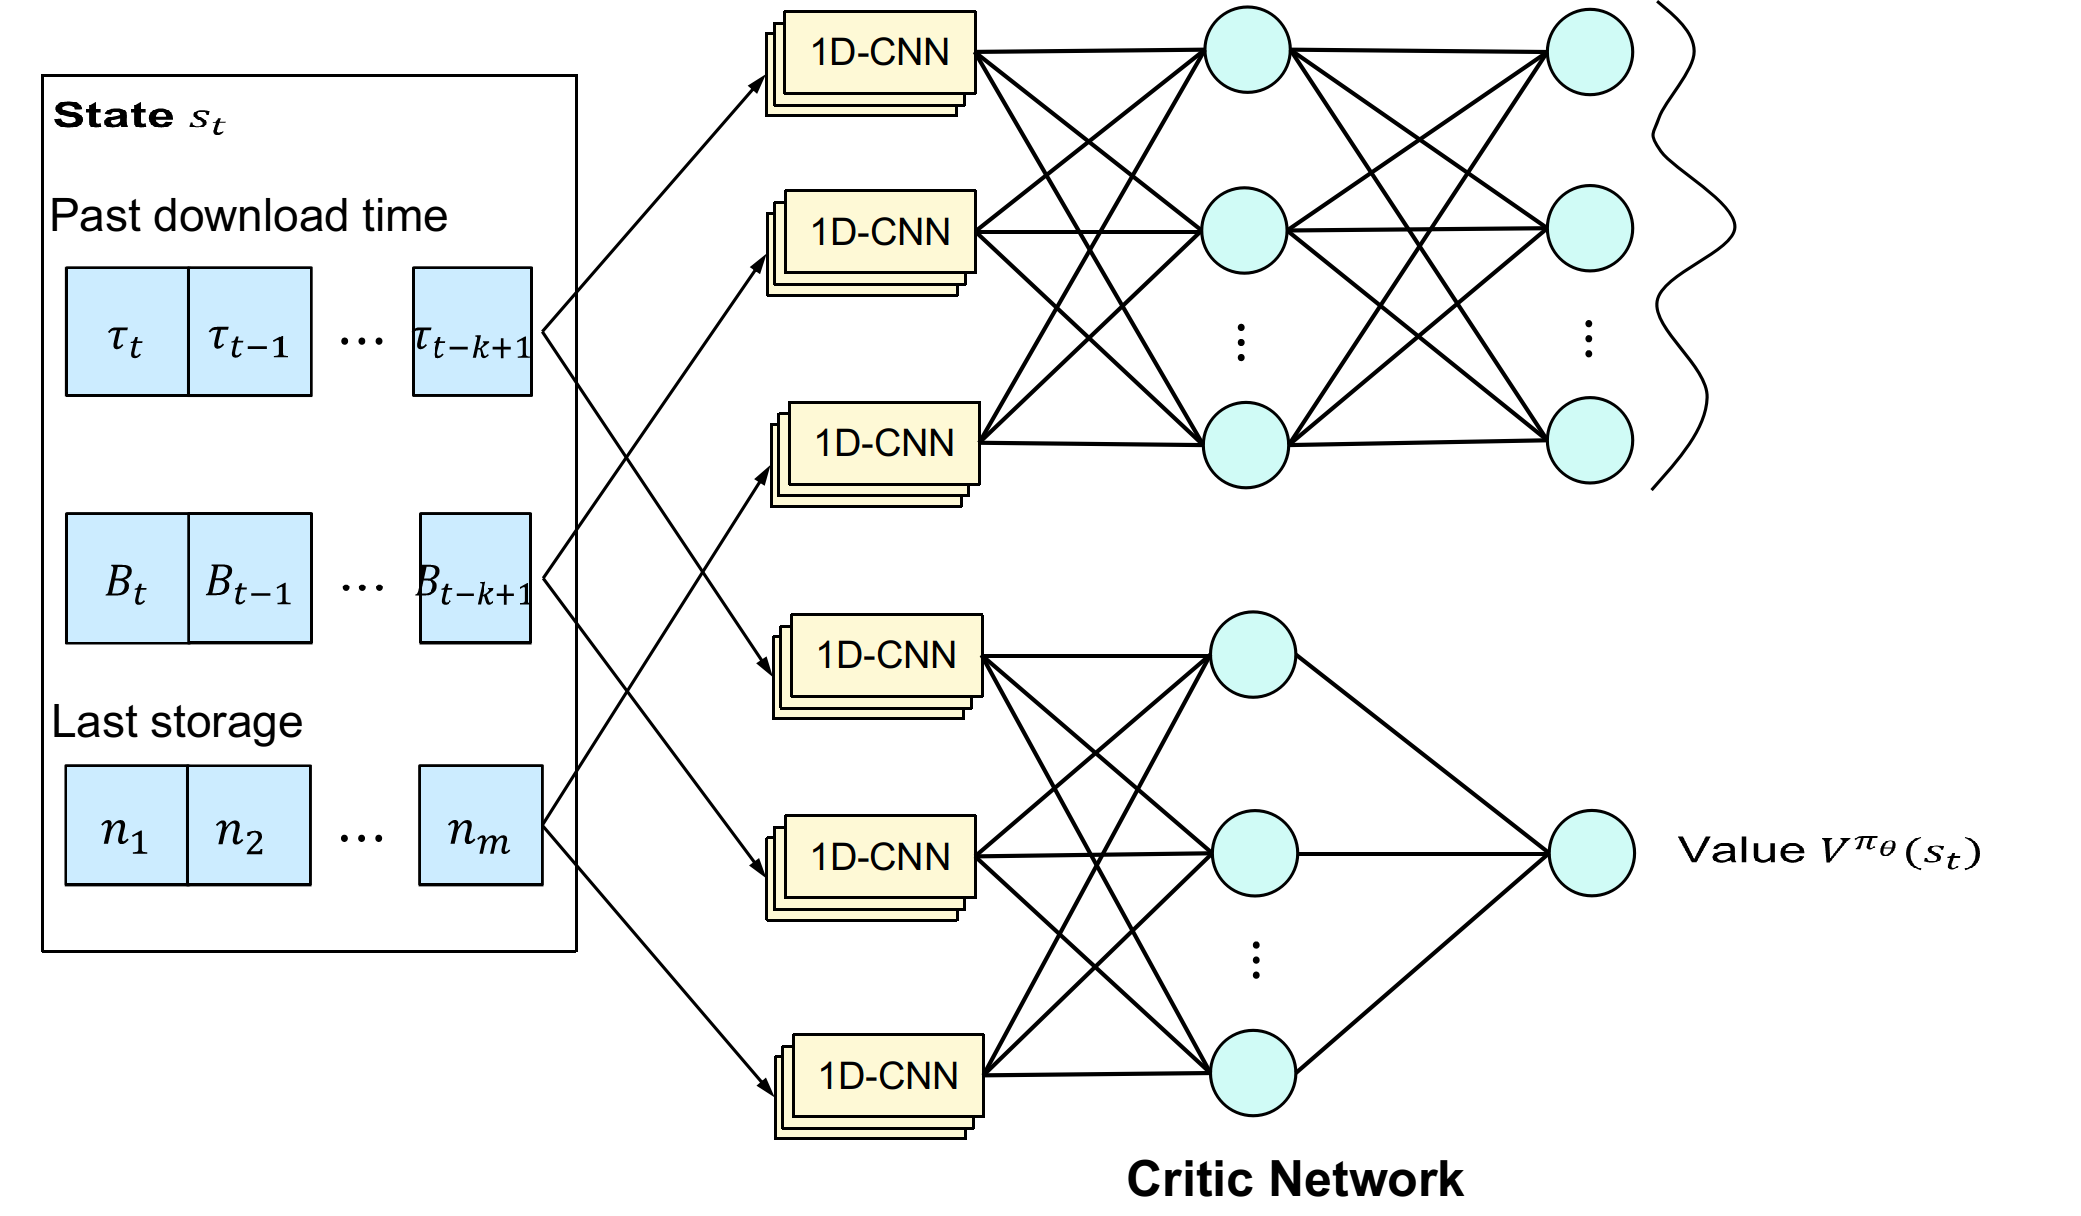
\includegraphics[width=0.8\linewidth]{a3c-network.png}
        \caption{The actor-Critic algorithms uses for \textsc{AutoCache}}
    \end{figure}
    
\end{section}

\begin{section}{Performance Evaluation}
    \label{exp}
    We obtain the real users' data from Google \cite{clusterdata:Reiss2011}, and the actual usage is directly borrowed from cooked data by \cite{Pensieve}. As the data trace following the format as: [timestamp (s), bandwidth (MBps)], we could collect enough data samples under different network conditions, and plot rather accurate CDF (Cumulative Distribution Function) graph versus the value with normalized service time. The experiments details are listed in the following sections. 
    
    \subsection{Simulation Setup}
    We firstly talk about the parameters setup we use and the data trace.
    We implement our algorithm with Tensorflow written in Python. The preliminary for the experiment environment is: Python 3.7+, Tensorflow 1.9+. Our program runs regardless of operating system, but we suggest Linux system for better compatibility. Our experiment following is carried out on Windows Subsystem for Linux (WLS) on Windows 10, and there are 4 parallel agents running on all the 4 CPU cores.

    Then we generate the random user request distribution with the following parameters. 
    The request interval is generated with Poisson Point Distribution with mean as 6 seconds ($\lambda=6$). There are total 6 files on the cloud for the user, and the popularity of files obeys Zipf's law over total files with parameter as $\alpha=1.07$.

    We choose the performance metric only with one cost: average service time. In order to highlight our algorithm performance, we also propose to compare the result from our DRL algorithm with that from heuristic algorithms. We adapt one classical offline algorithm, LRU for comparison. LRU refers to \textit{Least Recently Used}, which discards the least recently used items firstly in cache. The algorithm requires keeping track of the frequency of all the items, and performance passive caching only when the request is initiated.

    The comparison for statistics property of service delay will be discussed in the results section. By taking Google production data trace as evaluation test-bed, we expect our algorithm could outperform the simple heuristic algorithm.    

    \subsection{Results}
    Under the environment and parameters setup in the previous section, we firstly train the A3C neural network for actor and critic with training data. The training process is carried out in a pseudorandom way to enlarge the differences among all of the parallel agents. After enough epoch of training, we test our algorithm with the trained model over test data trace. For fairness, the comparison with LRU is over same data trace set.

    Then we compare \textsc{AutoCache} with classical algorithm LRU. The results for training traces with 1000 samples is shown in Figure \ref{fig:train}; and the results for test traces with 1000 samples is shown in Figure \ref{fig:test}.
    
    \begin{figure}[htp]
        \centering
        \subfloat[with training data trace]{
            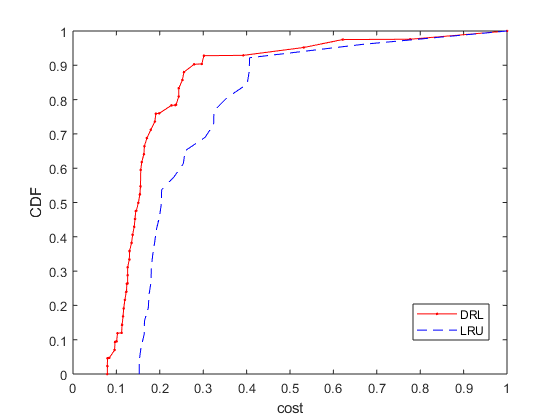
\includegraphics[width=0.45\linewidth]{training.png}
            \label{fig:train}
        }
        \hfill
        \subfloat[with test data trace]{
            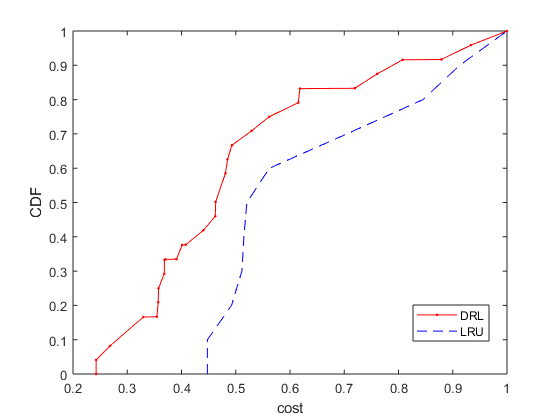
\includegraphics[width=0.45\linewidth]{testing.png}
            \label{fig:test}
        }
        \caption{The CDF of service delay of LRU and DRL algorithm under training and test data trace}
    \end{figure}

    According to the CDF graph, we could find that: whatever in training data trace or not, our algorithm \textsc{AutoCache} could always outperform the classical LRU algorithm as the distribution of service delay is rather prefer to lower side. The drop of average delay would vary from $10\%-15\%$.
\end{section}

\begin{section}{Conclusion}
    \label{summary}
    In this paper, we study one simplified scenario for edge network caching environment. We identify that the single-user-single-cache game could be separated into two phases, proactive caching and passive service, where the transition signal is the user's file request. In the proactive phase, we formulate one reinforcement learning problem and in the second phase we find one heuristic algorithm to efficiently 
    Then we develop our proactive caching prediction algorithm \textsc{AutoCache} with Tensorflow, and compare with classical passive caching algorithm LRU. Over large sample set under different network conditions, the CDF of service time shows that our algorithm could obviously outperform LRU, and the storage varies slowly with less bandwidth consumed.
\end{section}

% \subsubsection*{Acknowledgments}
% Thanks for the inspiration from \textit{Pensieve} the paper that we could make up this model. Thanks for Pro TAN Haisheng's description on basic caching problem.

% \section*{References}
\bibliographystyle{IEEEtran}
\bibliography{main.bib}

\end{document}
